\documentclass{article}
\usepackage{listings}
\usepackage{indentfirst}
\usepackage{url}
\usepackage{graphicx}
\usepackage{subfigure}
\usepackage{xcolor}



\title{Hanged Man Game}
\author{DP1-1 Eric, Rifile, Noel, Leo}


\begin{document}
    \setlength{\parindent}{0em}
    \lstset{
        backgroundcolor=\color{red!10!green!10!blue!10},%代码块背景色为浅灰色
        rulesepcolor= \color{gray}, %代码块边框颜色
        breaklines=true,  %代码过长则换行
        numbers=left, %行号在左侧显示
        numberstyle= \small,%行号字体
        keywordstyle= \color{blue},%关键字颜色
        commentstyle=\color{gray}, %注释颜色
        frame=shadowbox%用方框框住代码块
    }

    \maketitle
    \paragraph{Abstract}
    In our paper, we designed a computer game called "Hanged Man". We utilized top-down programming methodology, dividing our design into several modules. 
    
    This paper includes the structure of our design, flowchart and pseudocode of each module, and c++ program implementation.

    \newpage

    \tableofcontents
    \newpage

    \section{Introduction}
        Hanged Man is a game. One player enter the hardness, word, and hint, another player try characters and if the character he / she input is in the word, all same characters in the word would appear; if the character is NOT in the word, a stroke is added to a hanged man. When all the characters are tried out, player 2 win; when the hanged man are completely drawn, player 2 die.

        All the works of this project are uploaded to github repository \url{https://github.com/EricEricEricJin/Hanged-Man-Game.git](https://github.com/EricEricEricJin/Hanged-Man-Game.git}
    
    \newpage
    \section{Task assigning}
        \begin{table}[h]
            \begin{center}
                \begin{tabular}{|l|l|}
                    \hline
                    Task & Name \\ \hline
                    Structure chart & Leo \\ \hline
                    Flowchart & Rifile \\ \hline
                    Pseudocode & Eric \\ \hline
                    C++ implementation & Eric and Rifile \\ \hline
                    
                    Presentation & Rifile and Noel \\ \hline
                    Document & Eric \\ \hline                    
                \end{tabular}}
            \end{center}
        \end{table}

    \newpage

    \section{Design choice}
        \begin{enumerate}
            \item \textbf{Hardness and lives}
            Due to the relationship between 2 players is different, the probability for player 2 to think up the word is different. So we set three hardness in the game. Different hardness stands for different number of lives the player2 initially have, as shown in table below:
            
            \begin{table}[h]
                \begin{center}
                    \begin{tabular}{|l|l|}
                        \hline
                        Hardness & Initial lives \\ \hline
                        SIMPLE & 10 \\ \hline
                        MIDDLE & 9 \\ \hline
                        HARD & 8 \\ \hline
                    \end{tabular}
                \end{center}
            \end{table}

            \item \textbf{Represent the hanged man}
                In order to give player2 a better game experience, we draw the man with ascii characters. In this way, player2 can clearly know how many lives he / she still have.
                
        \end{enumerate}

    \newpage

    \section{Structure}
        % We used top-down design in our project as shown in \ref{structure_chart}

        \begin{figure}[htbp]

            \centering
            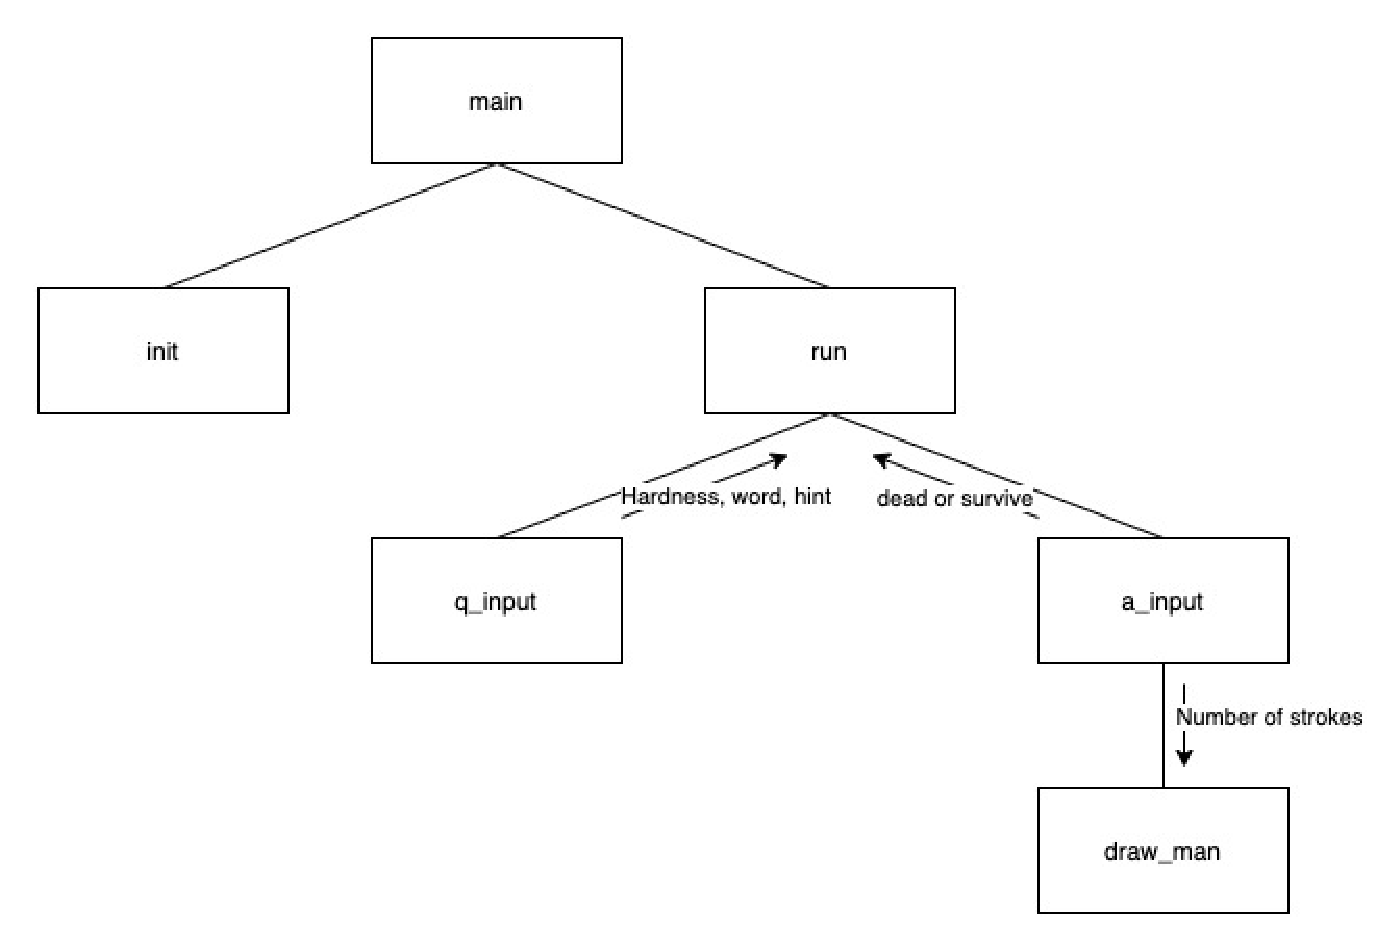
\includegraphics[height = 8cm]{structure.eps}
            \caption{Structure chart}
            \label{structure_chart}
        \end{figure}

    \newpage

    \section{Flowchart}
        \begin{figure}[htbp]
            \centering
            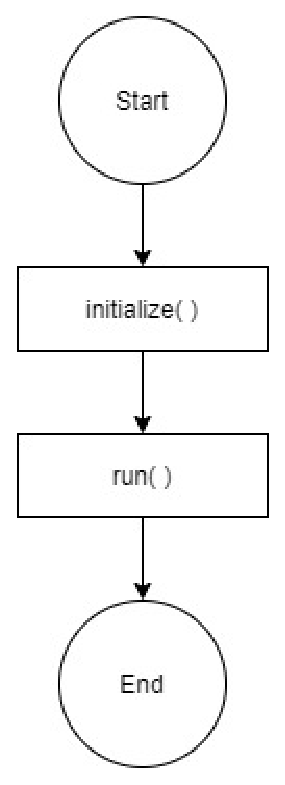
\includegraphics[height = 12cm]{flowchart/main.eps}
            \caption{main}
        \end{figure}

        \begin{figure}[htbp]
            \centering
            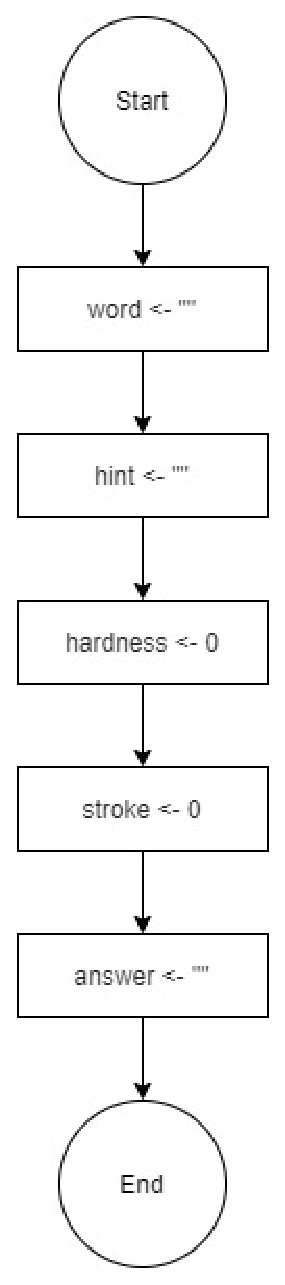
\includegraphics[height = 12cm]{flowchart/initialize.eps}
            \caption{initialize}
        \end{figure}
                    
        \begin{figure}[htbp]
            \centering
            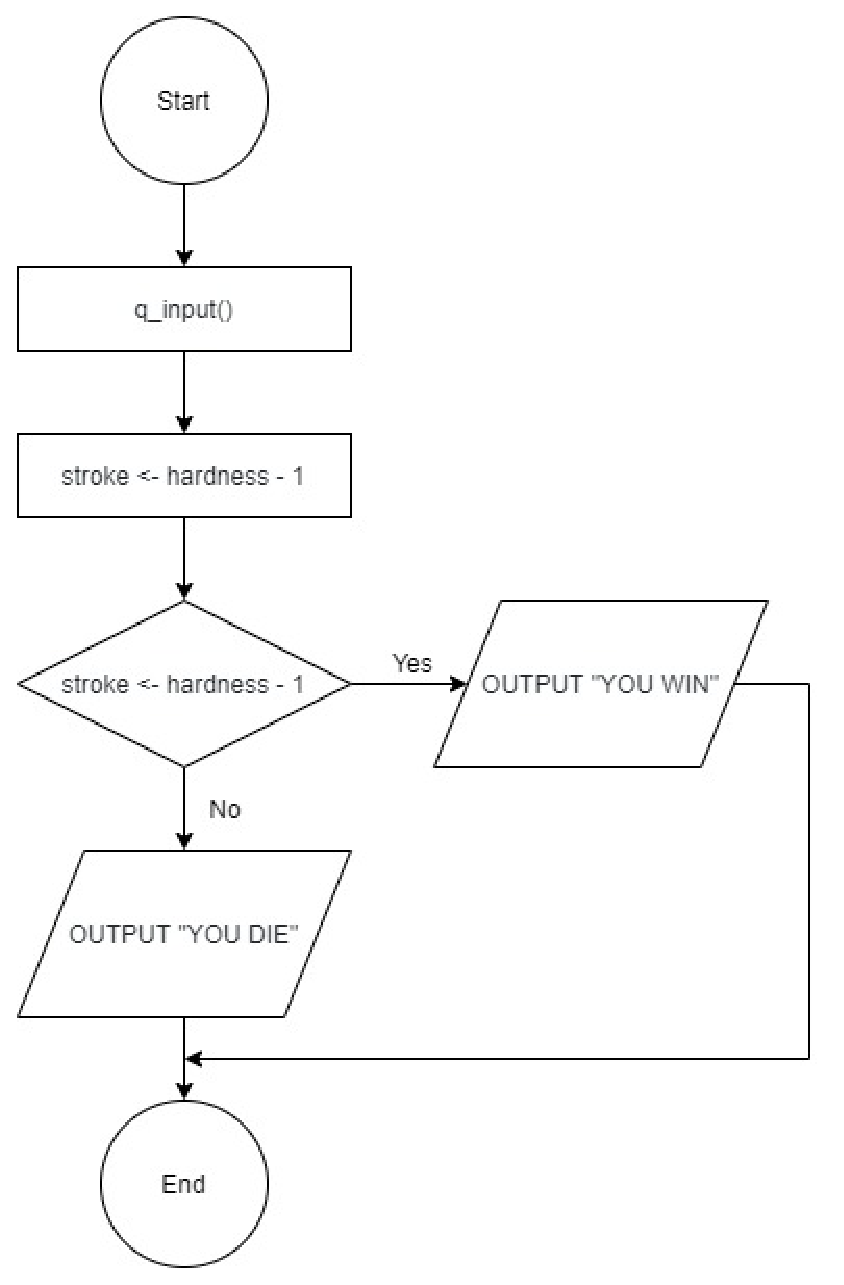
\includegraphics[height = 12cm]{flowchart/run.eps}
            \caption{run}
        \end{figure}

        \begin{figure}[htbp]
            \centering
            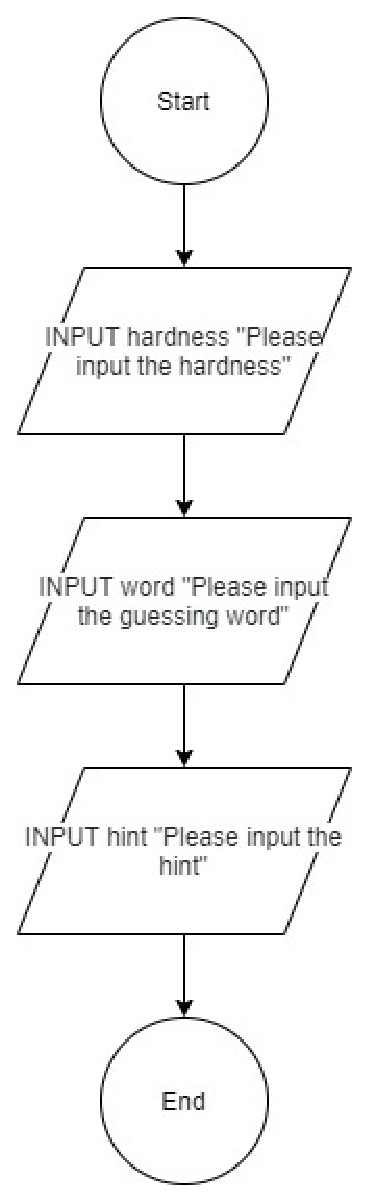
\includegraphics[height = 12cm]{flowchart/q_input.eps}
            \caption{q\_input}
        \end{figure}

        \begin{figure}[htbp]
            \centering
            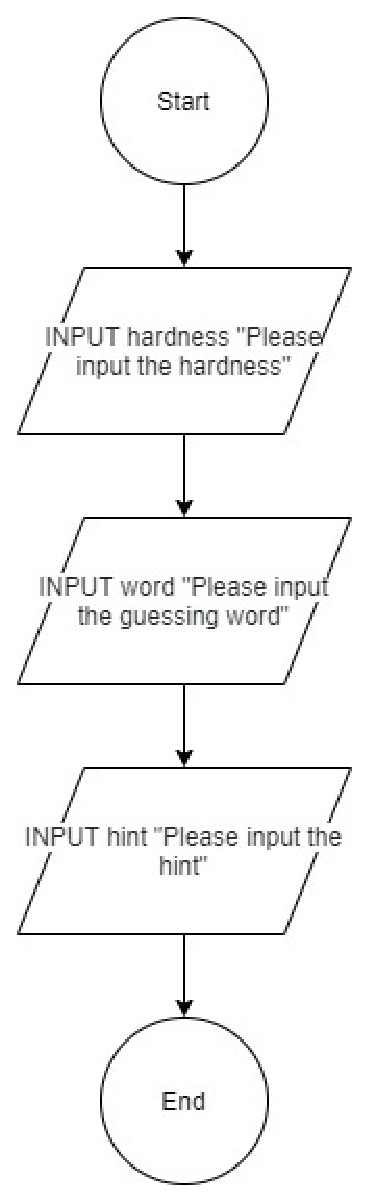
\includegraphics[height = 12cm]{flowchart/a_input.eps}
            \caption{a\_input}
        \end{figure}

        \begin{figure}[htbp]
            \centering
            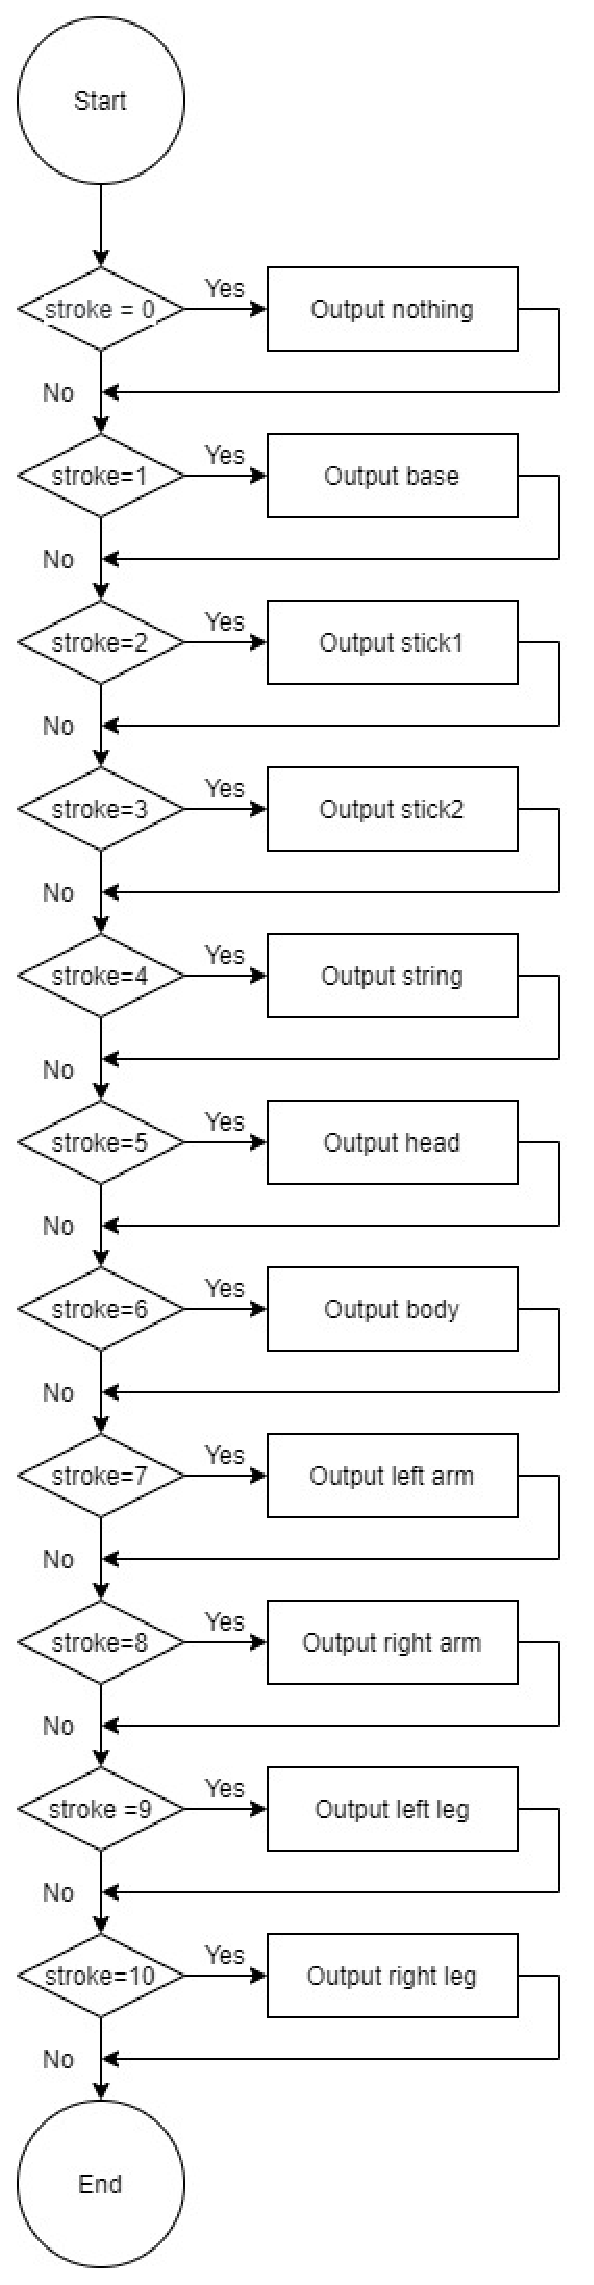
\includegraphics[height = 12cm]{flowchart/draw_man.eps}
            \caption{draw\_man}
        \end{figure}
        
    \newpage
    \section{Pseudocode}
        \textbf{main} 
        \begin{lstlisting}
initialize()
run()
        \end{lstlisting}
        \\

        \textbf{init} 
        \begin{lstlisting}
PROC initialize ()
    DECLARE word: STRING
    DECLARE hint: STRING
    DECLARE hardness: INTEGER
    DECLARE stroke: INTEGER
    DECLARE answer: STRING
    
    word <- ""
    hint <- ""
    hardness <- 0
    stroke <- 0
    answer <- ""
ENDPROC
        \end{lstlisting}
        \\

        \textbf{run}
        \begin{lstlisting}
PROC run()
    q_input()
    stroke <- hardness - 1
    IF a_input() = 1 THEN
        OUTPUT "YOU WIN"
    ELSE
        OUTPUT "YOU DIE"
    ENDIF
ENDPROC
        \end{lstlisting}
        \\

        \textbf{q\_input}
        \begin{lstlisting}
PROC q_input()
    INPUT hardness "Please input the hardness"
    INPUT word "Please input the guessing word"
    INPUT hint "Please input the hint"
ENDPROC 
        \end{lstlisting}
        \\

        \textbf{a\_input}
        \begin{lstlisting}
PROC a_input()
    DECLEAR key: CHARACTER
    DECLEAR i: INTEGER
    DECLEAR has_correct: BOOLEN
    key <- ""

    WHILE
        INPUT key
        has_correct <- 0
        FOR i <- 0 TO word.LENGTH
            IF word[i] = key THEN
                answer[i] <- key
                has_correct <- 1
            ENDIF
        ENDFOR
        OUTPUT answer
        IF has_correct = 0 THEN
            stroke <- stroke + 1
            draw_man(stroke)
            IF stroke >= LIVES THEN
                // loose
                RETURN 0;
            ENDIF
        ELIF answer = word THEN
            // win
            RETURN 1;
        ENDIF
    ENDWHILE
ENDPROC
        \end{lstlisting}
        \\

        \textbf{draw\_man}
        \begin{lstlisting}
PROC draw_man()
    IF stroke == 0 THEN
        OUTPUT 
            "
                

                



                
            "

    ELIF stroke == 1 THEN
        OUTPUT 
            "
                




                

                ********
            "

    ELIF stroke == 2 THEN
        OUTPUT 
            "
                *
                *
                *
                *
                *
                *
                *
                ********
            "

    ELIF stroke == 3 THEN
        OUTPUT 
            "
                *****
                *
                *
                *
                *
                *
                *
                ********
            "

    ELIF stroke == 4 THEN
        OUTPUT 
            "
                *****
                *   *
                *
                *
                *
                *
                *
                ********
            "

    ELIF stroke == 5 THEN
        OUTPUT 
            "
                *****
                *   *
                *  * *
                *   *
                *
                *
                *
                ********
            "

    ELIF stroke == 6 THEN
        OUTPUT 
            "
                *****
                *   *
                *  * *
                *   *
                *   *
                *   *
                *
                ********
            "
    ELIF stroke == 7 THEN
        OUTPUT
            "
                *****
                *   *
                *  * *
                *   *
                *  **
                *   *
                *
                ********
            "
    ELIF stroke == 8 THEN
        OUTPUT
            "
                *****
                *   *
                *  * *
                *   *
                *  ***
                *   *
                *
                ********
            "

    ELIF stroke == 9 THEN
        OUTPUT
            "
                *****
                *   *
                *  * *
                *   *
                *  ***
                *   *
                *  *
                ********
            "   

    ELIF stroke == 10 THEN
        OUTPUT
            "
                *****
                *   *
                *  * *
                *   *
                *  ***
                *   *
                *  * *
                ********
            "    
    ENDIF
ENDPROC
        \end{lstlisting}
    
    \newpage

    \section{Identifier table}
        \begin{table}[h]
            \begin{center}
                \begin{tabular}{|l|l|l|}
                    \hline
                    Name & Type & Description \\ \hline
                    word & STRING & the word input by player 1 \\ \hline
                    hint & STRING & hint input by player 1 offered to player 2 \\ \hline
                    hardness & INTEGER & game hardness input by player 1 \\ \hline
                    stroke & INTEGER & stroke of the hanged man \\ \hline
                    answer & STRING & characters input by player 2 \\ \hline
                    key & CHARACTER & key pressed by player 2 \\ \hline
                    i & INTEGER & counter \\ \hline
                    has_correct & BOOLEN & the character exist in the word or not \\ \hline
                \end{tabular}
            \end{center}
            \caption{Identifier table}
        \end{table}
    
    \newpage
    \section{C++ implementation}
        \textbf{hanged\_man.h}
        \begin{lstlisting}[language={cpp}]
#ifndef _H_M__
#define _H_M__

#define WINDOW_H 24
#define WINDOW_W 80

#define WORD_MAX_LEN 20
#define HINT_MAX_LEN 100

#define LIVES 10

#include <cstdio>
#include <cstdlib>
#include <curses.h>

struct string {
    char* text;
    int len;
};

class hangedMan {
    private:
        WINDOW* main_win;
        WINDOW* man_win;
        WINDOW* IO_win;

        int q_input_stage;
        int hardness;
        string* hint;
        string* word;
        string* answer;

        int stroke;

        
        int restart;

        void draw_man();
        int q_input(int key_val);
        int a_input(int key_val);
        int strcomp(char* s1, char* s2, int len);
        void die();
        void win();
        void del();
        int rst_input(int key_val);
        string* init_str(int len, char chr);
        void free_str(string* str);

    public:
        hangedMan();
        void run();

};
#endif
        \end{lstlisting}

        \textbf{main.cpp}
        \begin{lstlisting}[language={cpp}]
#include "hanged_man.h"

using namespace std;
int main() {
    hangedMan H;
    H.run();
}
        \end{lstlisting}

        \textbf{init.cpp}
        \begin{lstlisting}[language={cpp}]
/**
* Function: init
* Description: initialize as the class is instantiated
* Parameter: None
* Return: None
*/

#include "hanged_man.h"

hangedMan::hangedMan() {
    main_win = initscr();
    man_win = subwin(main_win, LINES, int(COLS / 2), 0, int(COLS / 2));
    IO_win = subwin(main_win, LINES, int(COLS / 2), 0, 0);
    // cbreak();
    noecho();
}
        \end{lstlisting}

        \textbf{run.cpp}
        \begin{lstlisting}[language={cpp}]
/**
* Function: run
* Description: the main loop of the game
* Parameter: None
* Return: None
*/

#include "hanged_man.h"

void hangedMan::run() {
    word = init_str(WORD_MAX_LEN, 0);
    hint = init_str(HINT_MAX_LEN, 0);
    q_input_stage = 0;
    hardness = 0;
    stroke = 0;
    restart = 0;
    
    wclear(main_win);
    wclear(man_win);
    wclear(IO_win);

    box(main_win, ACS_VLINE, ACS_HLINE);

    int key_val = 0;
    q_input_stage = 0;
    while (1) {
        
        if (q_input(key_val) == 1) {
            break;
        }
        key_val = getch();
    }
    
    wclear(main_win);
    box(main_win, ACS_VLINE, ACS_HLINE);
    box(man_win, ACS_VLINE, ACS_HLINE);
    box(IO_win, ACS_VLINE, ACS_HLINE);

    stroke += hardness - 1;
    answer = init_str(word -> len, 95);

    wprintw(IO_win, answer -> text);
    key_val = 0;

    int brk = 0;
    while (1) {
        if (brk == 1) {
            break;
        }
        switch (a_input(key_val)) {
            case 1:
                win();
                brk = 1;
                break;
            case -1:
                brk = 1;
                die();
                break;
            default:
                key_val = getch();
                break;
        }
    }

    // restart or quit
    getch();
    key_val = 0;
    restart = 0;
    while (1) {
        if (rst_input(key_val) == 1) {
            if (restart == 0) {
                del();
            } else if (restart == 1) {
                del();
                run();
            }
            break;
        }
        key_val = getch();
    }
}
        \end{lstlisting}

        \textbf{a\_input.cpp}
        \begin{lstlisting}[language={cpp}]
/**
* Function: a_input
* Description: the player input the answer
* Parameter: key_val
* Return: die(-1) or win(1) or unfinished(0)
*/

#include "hanged_man.h"

int hangedMan::a_input(int key_val) {
    if (key_val != 0) {
        int hasCorrect = 0;
        for (int i = 0; i < word -> len; i++) {
            if (*(word -> text + i) == key_val) {
                hasCorrect = 1;
                *(answer -> text + i) = key_val;
            }
        }
        
        if (hasCorrect == 0) {
            stroke += 1;
        }
    }
    wclear(IO_win);
    box(IO_win, ACS_VLINE, ACS_HLINE);
    wmove(IO_win, int(LINES / 2), 5);
    wprintw(IO_win, answer -> text);
    wmove(IO_win, int(LINES / 2) + 2, 5);
    wprintw(IO_win, "Hint:");
    wmove(IO_win, int(LINES / 2) + 3, 5);
    wprintw(IO_win, hint -> text);
    wrefresh(IO_win);
    draw_man();
    
    if (stroke >= 10) {
        // dead
        return -1;
    } else if (strcomp(answer -> text, word -> text, word -> len) == 1) {
        return 1;
    }
    return 0;
}
        \end{lstlisting}

        \textbf{q\_input.cpp}
        \begin{lstlisting}
/**
* Function: q_input
* Description: input of question
* Parameter: key_val
* Return: 0 not decide or 1 decided
*/

#include "hanged_man.h"

int hangedMan::q_input(int key_val) {
    wclear(main_win);
    box(main_win, ACS_VLINE, ACS_HLINE);
    if (key_val == 9) {
        q_input_stage += 1;
        if (q_input_stage > 3) {
            q_input_stage = 0;
        }
    } else {
        switch (q_input_stage) {
            case 0: // hardness
                switch (key_val) {
                    case 49:
                        hardness = 1;
                        break;
                    case 50:
                        hardness = 2;
                        break;
                    case 51:
                        hardness = 3;
                        break;
                }
                break;
            
            case 1: // word
                if (key_val >= 97 && key_val <= 122) {
                    if (word -> len < WORD_MAX_LEN) {
                        *(word -> text + word -> len) = key_val;
                        word -> len += 1;
                    }
                } else if (key_val == 127) { // delete
                    if (word -> len > 0) {
                        *(word -> text + word -> len - 1) = 0;
                        word -> len -= 1;
                    }
                }
                break;

            case 2: // Hint
                if (key_val >= 97 && key_val <= 122) {
                    if (hint -> len < HINT_MAX_LEN) {
                        *(hint -> text + hint -> len) = key_val;
                        hint -> len += 1;
                    }
                } else if (key_val == 127) { // delete
                    if (hint -> len > 0) {
                        *(hint -> text + hint -> len - 1) = 0;
                        hint -> len -= 1;
                    }
                }
                break;

            case 3:
                if (key_val == 10) {
                    return 1;
                }

            default:
                break;
        }
    }

    // show
    wmove(main_win, 1, 10);
    wprintw(main_win, "Hardness");

    wmove(main_win, 2, 10);
    switch (hardness) {
        case 1:
            wprintw(main_win, "SIMPLE");
            break;
        case 2:
            wprintw(main_win, "MIDDLE");
            break;
        case 3:
            wprintw(main_win, "HARD");
            break;
        default:
            break;
    }
    
    wmove(main_win, 3, 10);
    wprintw(main_win, "Word");

    wmove(main_win, 4, 10);
    wprintw(main_win, word -> text);

    wmove(main_win, 5, 10);
    wprintw(main_win, "Hint");

    wmove(main_win, 6, 10);
    wprintw(main_win, hint -> text);

    wmove(main_win, 7, 10);
    wprintw(main_win, "Finish");

    wmove(main_win, int(q_input_stage * 2 + 1), 1);
    wprintw(main_win, "->");
    return 0;
}
        \end{lstlisting}

        \textbf{rst\_input.cpp}
        \begin{lstlisting}[language={cpp}]
/**
* Function: rst_input
* Description: get user's restart or quit input after game end
* Parameter: key_val
* Return: 0: not decide, 1: decided
*/

#include "hanged_man.h"

int hangedMan::rst_input(int key_val) {
    int rt = 0;
    switch (key_val) {
        case 9:
            restart += 1;
            if (restart > 1) {
                restart = 0;
            }
            rt = 0;
            break;
        case 10:
            rt = 1;
            break;
        default:
            rt = 0;
            break;
    }

    wclear(main_win);
    wmove(main_win, int(LINES / 2) + 5, int(COLS / 2));
    wprintw(main_win, "RESTART");
    wmove(main_win, int(LINES / 2) + 6, int(COLS / 2));
    wprintw(main_win, "QUIT");
    wmove(main_win, int(LINES / 2) + 6 - restart, int(COLS / 2) - 5);
    wprintw(main_win, "-->");
    wrefresh(main_win);

    return rt;
}
        \end{lstlisting}
        
        \textbf{draw\_man.cpp}
        \begin{lstlisting}[language={cpp}]
/**
* Function: draw_man
* Description: draw the man
* Parameter: None
* Return: None
*/

#include "hanged_man.h"

void hangedMan::draw_man() {
    wclear(man_win);
    box(man_win, ACS_VLINE, ACS_HLINE);
    // wprintw(man_win, "%d", stroke);
    int counter = 0;
    if (counter >= stroke) {
        wrefresh(man_win);
        return;
    }

    wmove(man_win, LINES - 5, 5);
    whline(man_win, 42, 10);

    counter += 1;
    if (counter >= stroke) {
        wrefresh(man_win);
        return;
    }
    
    wmove(man_win, 5, 5);
    wvline(man_win, 42, (LINES - 10));

    counter += 1;
    if (counter >= stroke) {
        wrefresh(man_win);
        return;
    }

    whline(man_win, 42, 8);

    counter += 1;
    if (counter >= stroke) {
        wrefresh(man_win);
        return;
    }

    wmove(man_win, 5, 13);
    wvline(man_win, 42, 4);

    counter += 1;
    if (counter >= stroke) {
        wrefresh(man_win);
        return;
    }

    wmove(man_win, 7, 12);
    whline(man_win, 42, 3);
    wvline(man_win, 42, 3);
    wmove(man_win, 9, 12);
    whline(man_win, 42, 3);
    wmove(man_win, 7, 14);
    wvline(man_win, 42, 3);


    counter += 1;
    if (counter >= stroke) {
        wrefresh(man_win);
        return;
    }

    wmove(man_win, 8, 13);
    wvline(man_win, 42, 4);


    counter += 1;
    if (counter >= stroke) {
        wrefresh(man_win);
        return;
    }
    
    wmove(man_win, 10, 10);
    whline(man_win, 42, 3);

    counter += 1;
    if (counter >= stroke) {
        wrefresh(man_win);
        return;
    }

    wmove(man_win, 10, 13);
    whline(man_win, 42, 4);

    counter += 1;
    if (counter >= stroke) {
        wrefresh(man_win);
        return;
    }

    wmove(man_win, 12, 12);
    wvline(man_win, 42, 2);

    counter += 1;
    if (counter >= stroke) {
        wrefresh(man_win);
        return;
    }

    wmove(man_win, 12, 14);
    wvline(man_win, 42, 2);
    counter += 1;
    if (counter >= stroke) {
        wrefresh(man_win);
        return;
    }
}            
        \end{lstlisting}
        
        \textbf{win.cpp}
        \begin{lstlisting}[language={cpp}]
/**
* Function: win
* Description: called after player2 win
* Parameter: None
* Return: None
*/

#include "hanged_man.h"

void hangedMan::win() {
    wclear(main_win);
    wmove(main_win, int(LINES / 2), int(COLS / 2) - 5);
    wprintw(main_win, "YOU WIN");
    box(main_win, ACS_VLINE, ACS_HLINE);
    wrefresh(main_win);
}
        \end{lstlisting}

        \textbf{die.cpp}
        \begin{lstlisting}[language={cpp}]
/**
* Function: die
* Description: what to do after die
* Parameter: None
* Return: None
*/

#include "hanged_man.h"

void hangedMan::die() {
    wclear(IO_win);
    wmove(IO_win, int(LINES / 2), int(COLS / 4));
    wprintw(IO_win, "YOU DIE!");
    
    stroke = 5;
    draw_man();

    wmove(man_win, 13, 13);
    wvline(man_win, 42, 4);

    
    wmove(man_win, 15, 10);
    whline(man_win, 42, 3);


    wmove(man_win, 15, 13);
    whline(man_win, 42, 4);


    wmove(man_win, 17, 12);
    wvline(man_win, 42, 2);

    wmove(man_win, 17, 14);
    wvline(man_win, 42, 2);
    
    box(IO_win, ACS_VLINE, ACS_HLINE);
    wrefresh(man_win);
    wrefresh(IO_win);
}
        \end{lstlisting}

        \textbf{del.cpp}
        \begin{lstlisting}[language={cpp}]
/**
* Function: del
* Description: free the allocated memory
* Parameter: None
* Return: None
*/

#include "hanged_man.h"

void hangedMan::del() {
    endwin();
    free_str(word);
    free_str(hint);
    free_str(answer);
}
        \end{lstlisting}

        \textbf{init\_free\_str.cpp}
        \begin{lstlisting}[language={cpp}]
#include "hanged_man.h"

/**
    * Function: init_str
    * Description: initizlize a string structure
    * Parameter: string max length, initialize character
    * Return: string* of the string.
*/
string* hangedMan::init_str(int len, char chr) {
    string* str;
    str = (string*)malloc(sizeof(string));
    str -> text = (char*)malloc(sizeof(char) * len);
    for (int i = 0; i < len; i++) {
        *(str -> text + i) = chr;
    }
    str -> len = 0;
    return str;
}

/**
    * Function: free_str
    * Description: free the string structure
    * Parameter: string* string
    * Return: None
*/
void hangedMan::free_str(string* str) {
    free(str -> text);
    free(str);
}
        \end{lstlisting}

        \textbf{strcomp.cpp}
        \begin{lstlisting}[language={cpp}]
/**
* Function: strcomp
* Description: use to compare two string which have same length
* Parameter: string1, string2, length
* Return: 0 not smae or 1 same
*/

#include "hanged_man.h"

int hangedMan::strcomp(char* s1, char* s2, int len) {
    int same = 1;
    for (int i = 0; i < len; i++) {
        if (*(s1 + i) != *(s2 + i)) {
            same = 0;
        }
    }
    return same;
}
        \end{lstlisting}
    
    \newpage
    \section{Testing of implementation}
        \textbf{Compile environment} \\
        Mac OS X 10.15, g++ version 4.2.1, with curses lib installed

        \textbf{Makefile} \\
        \begin{lstlisting}
main:
g++ -o hanged_man.out main.cpp init.cpp run.cpp draw_man.cpp a_input.cpp q_input.cpp strcomp.cpp die.cpp win.cpp del.cpp rst_input.cpp init_free_str.cpp -l curses
        \end{lstlisting}

        \textbf{Running environment} \\
        Mac OS X 10.15, terminal window with size 80 cols and 24 rows

        \textbf{Testing results}
        \begin{figure}[htbp]
            \centering
            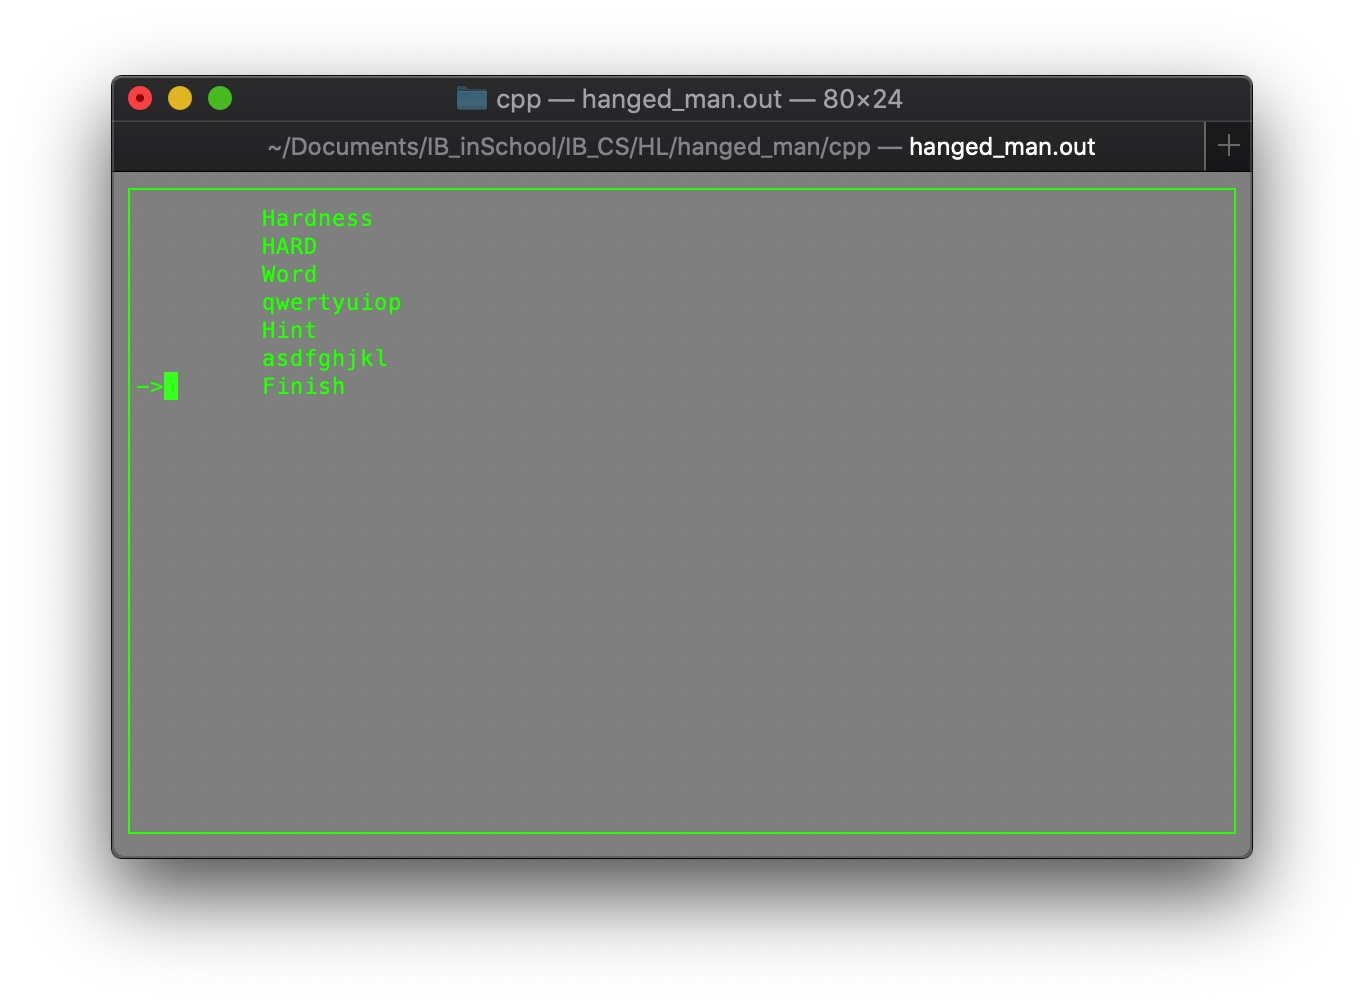
\includegraphics[height = 5cm]{testing/test_1.eps}
            \caption{Player 1 input hardness, word, and hint}
            \label{}
        \end{figure}

        \begin{figure}[htbp]
            \centering
            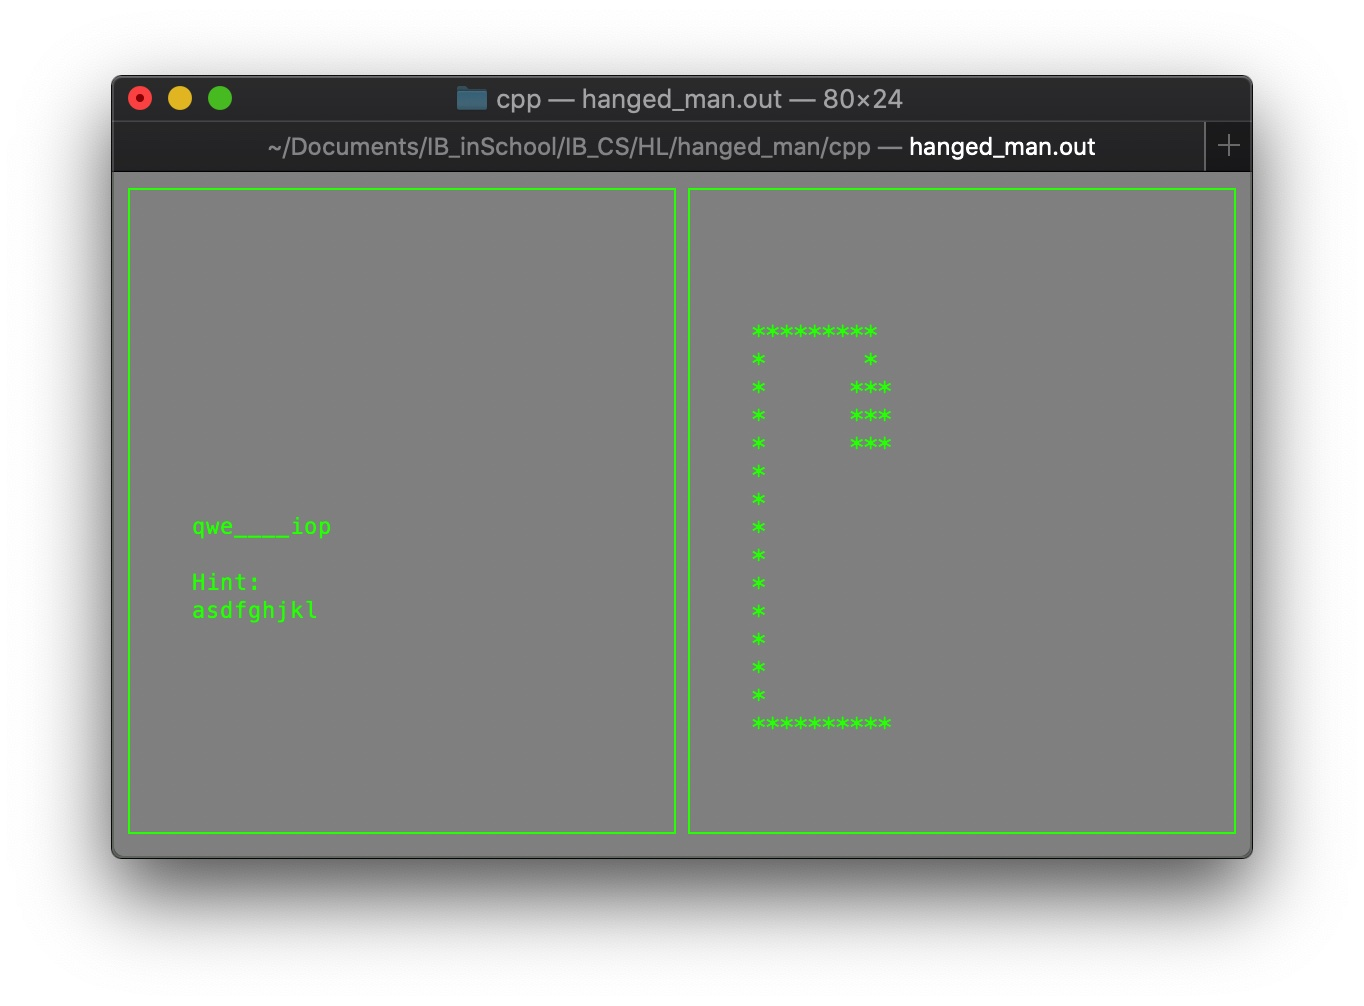
\includegraphics[height = 5cm]{testing/test_2.eps}
            \caption{Player 2 input answer}
            \label{}
        \end{figure}

        \begin{figure}[htbp]
            \centering
            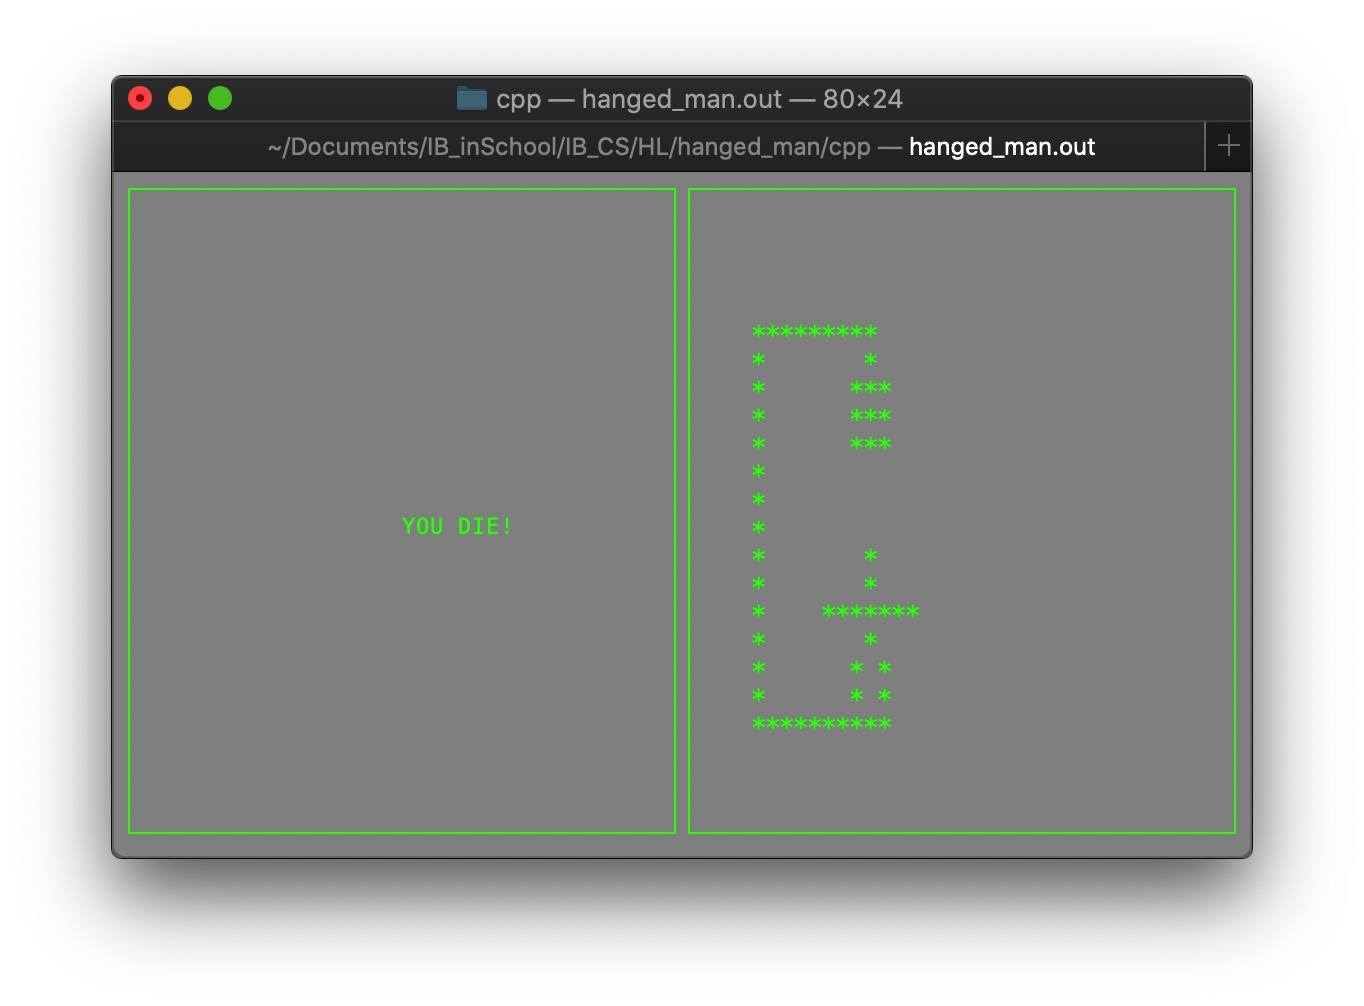
\includegraphics[height = 5cm]{testing/test_3.eps}
            \caption{Player 2 pass away}
            \label{}
        \end{figure}

        \begin{figure}[htbp]
            \centering
            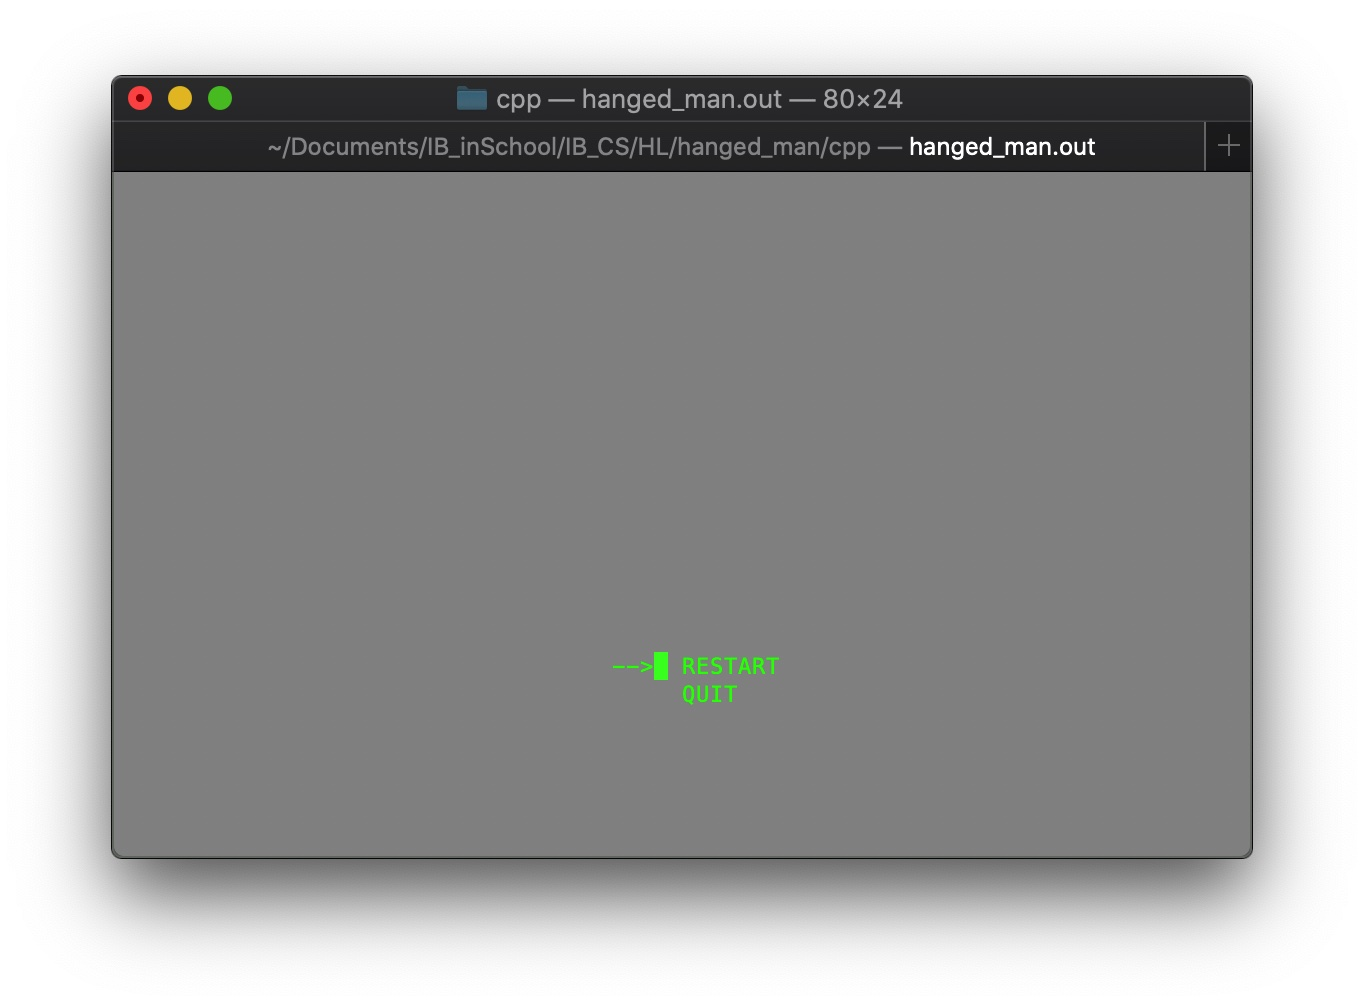
\includegraphics[height = 5cm]{testing/test_4.eps}
            \caption{Quit or restart}
            \label{}
        \end{figure}

        \begin{figure}[htbp]
            \centering
            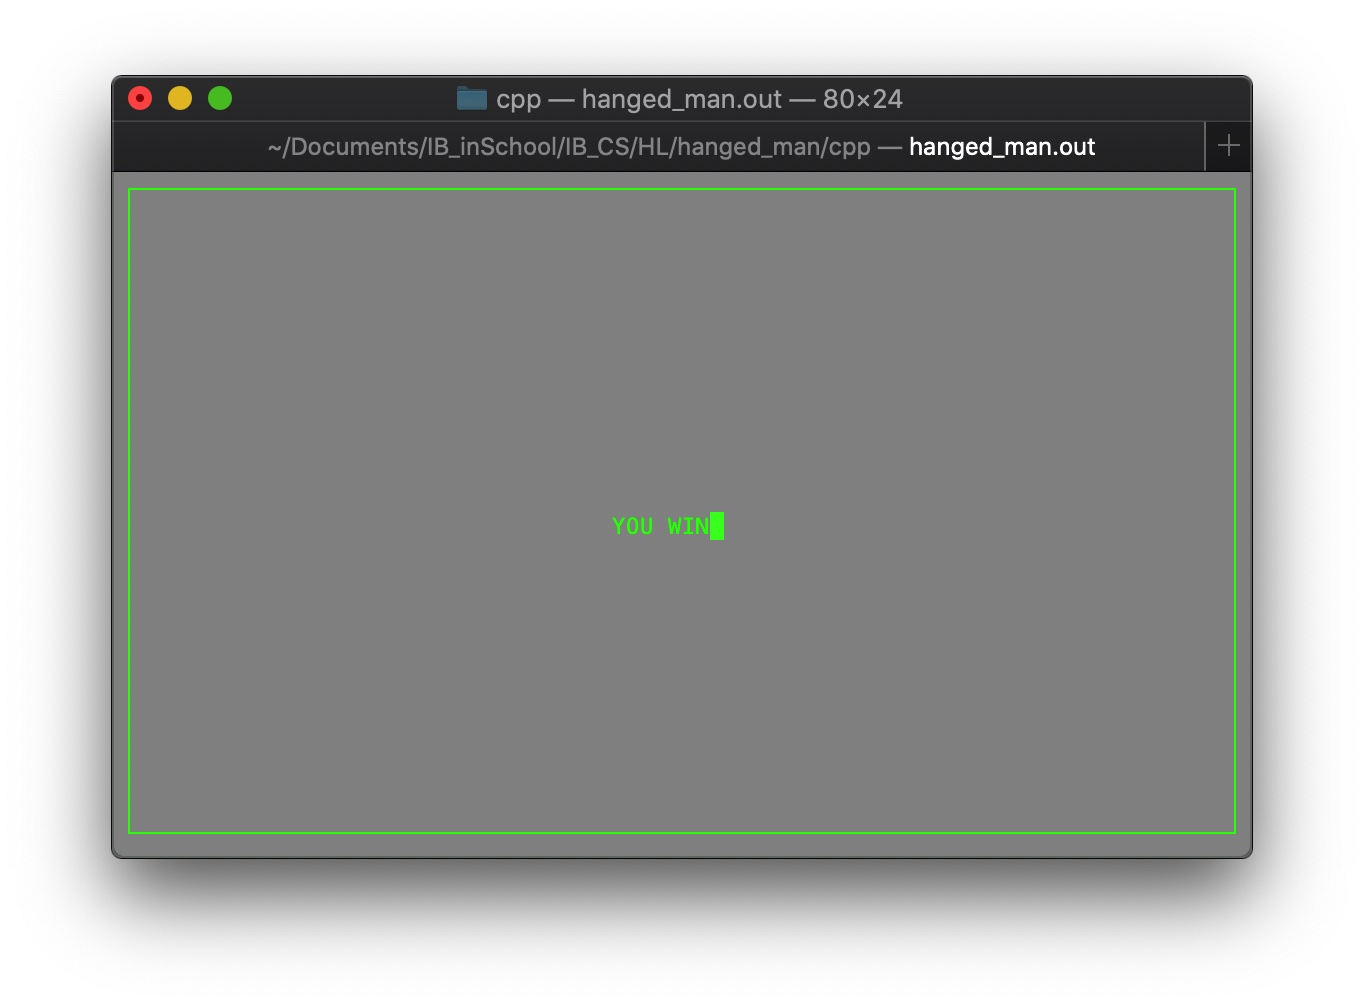
\includegraphics[height = 5cm]{testing/test_5.eps}
            \caption{Player 2 survive}
            \label{}
        \end{figure}
\end{document}
